\documentclass{article}

% if you need to pass options to natbib, use, e.g.:
% \PassOptionsToPackage{numbers, compress}{natbib}
% before loading nips_2018

% ready for submission
% \usepackage{nips_2018}

% to compile a preprint version, e.g., for submission to arXiv, add
% add the [preprint] option:
\usepackage[preprint]{nips_2018}

% to compile a camera-ready version, add the [final] option, e.g.:
% \usepackage[final]{nips_2018}

% to avoid loading the natbib package, add option nonatbib:
% \usepackage[nonatbib]{nips_2018}

\usepackage[utf8]{inputenc} % allow utf-8 input
\usepackage[T1]{fontenc}    % use 8-bit T1 fonts
\usepackage{hyperref}       % hyperlinks
\usepackage{url}            % simple URL typesetting
\usepackage{booktabs}       % professional-quality tables
\usepackage{amsfonts}       % blackboard math symbols
\usepackage{nicefrac}       % compact symbols for 1/2, etc.
\usepackage{microtype}      % microtypography
\usepackage{amsmath}
\usepackage{graphicx}
\usepackage[linesnumbered,ruled]{algorithm2e}

\title{Statistical generation of hand-written digits via analysis of learned latent representations}

% The \author macro works with any number of authors. There are two
% commands used to separate the names and addresses of multiple
% authors: \And and \AND.
%
% Using \And between authors leaves it to LaTeX to determine where to
% break the lines. Using \AND forces a line break at that point. So,
% if LaTeX puts 3 of 4 authors names on the first line, and the last
% on the second line, try using \AND instead of \And before the third
% author name.

\author{
  Ernesto Vargas Aguilar \\
  \texttt{vargasaguila@wisc.edu} \\
   \And
   Cong (Frank) Gu \\
   \texttt{cgu38@wisc.edu} \\
   \And
   Yunchan Clemence Lee \\
   \texttt{ylee642@wisc.edu} \\
}

\begin{document}
% \nipsfinalcopy is no longer used

\maketitle

\begin{abstract}
Variational Autoencoders learn the latent representation space of the input domain by learning to compress to and decompress from a stochastic latent representation space. This allows the information contained in the sample to be compressed into a lower dimension. Therefore, when used on classifiable dataset, it can retain the classification factors when transformed into the latent vector. By learning the conditional distribution within the latent space of each label sets within the domain, it is possible to perform categorical generation of artificial samples. In this work, we study the MNIST dataset and demonstrate that even a simple statistical analysis can result in a high-accuracy generative model.
\end{abstract}

\section{Introduction}

A generative model is a form of unsupervised learning whose goal is to use existing 
samples in the domain of interest to learn the defining characteristics of the domain,
and to use this knowledge to generate artificial samples that mimic these characteristics.
Once trained, a typical generative model uses techniques such as noise sampling and vector arithmetic
to modify existing or generate entirely new examples that are visually similar to the real instances of the domain.
In practical terms, generative models increasingly have more applications in creative fields like video game design, 
painting and visual art, music and poetry. \par

 Recent advances have given rise to a proliferation of research on generative models. Notable approaches include Variational AutoEncoders (VAEs) and Generative Adversarial Networks (GANs). VAEs leverage a highly compressed latent representation to extract key attributes of the input by learning its distribution, it has a impressive performance in accurately reconstructing the data space from lower dimensional space, making it an efficient candidate for generating new and diverse outputs from the same distribution. On the other hand, GAN models follow a 2-player min-max game theory to generate realistic, novel outputs, with both generator and discriminator improve their accuracy overtime.\par
 
A small subset of these approaches have focused on extending the traditional approaches to a supervised learning setting, training models using both the instances and the labels, to be able to conditionally generate samples depending on an input mapping to the label space. For example, Yan et al. leverages Bayesian inference using energy minimization approach for posterior inference in VAE. They conditioned on distinct visual attribute labels learned from facial images to allow for realistic image generation\cite{Yan}.  \par

In this work, we address the problem of conditional generation. We will describe traditional approach to VAEs (\hyperref[sec:background]{Section 2}), present novel approach to conditional generation (\hyperref[sec:proposal]{Section 3}), evaluate learned latent representation (\hyperref[sec:experiments]{Section 4}) and discuss related work (\hyperref[sec:related]{Section 5}).

\section{Background}
\label{sec:background}
\subsection{Variational Autoencoders}

A variational autoencoder (VAE) consists of two networks, encoder and decoder. The encoder
takes in samples in the domain of interest, and outputs a distribution in a lower dimensional
latent space \cite{Kingma2}. The decoder samples from this distribution and decodes the latent representation
back into data space. Specifically, the latent representation z is a sample from the Gaussian
probability density defined by the output of the encoder $q_\theta(\mathbf{z}|\mathbf{x})$, and
the final output of the VAE is a reconstruction $p_\theta(\mathbf{x}|\mathbf{z})$ of the original input 
from the sample z. \par
The objective function for training a VAE consists of two parts. First, the reconstruction loss measures how much the reconstructed output from the decoder differs from the original input. The second term is a regularizer measuring the similarity, or conversely divergence, between the encoded distribution $q_\theta(\mathbf{z}|\mathbf{x})$ and the given prior $p(z)$. The regularization term forces the representations of each structurally distinct group to be sufficiently diverse, leading to the network's ability to discern meaningful structures/patterns. A classical implementation of such loss function is the ELBO loss.
\begin{equation} 
l_i(\theta, \varphi) = - E_{z~q_\theta(z|x_i)} [\log{p_\theta(x_i|z)}]+KL(q_\theta(z|x_i)||p(z))
\end{equation}

\section{Proposed Method}
\label{sec:proposal}
\subsection{Motivation}

Variational Autoencoders learn the structure of the latent space given a prior distribution of the vector that represent the input in the latent space. Typically much smaller in dimension that the input, it has been observed that the latent structure can succinctly store information on distinguishing features of the inputs. Therefore, given a domain whose sample space can be classified into distinct subsets, it is probable that each of these subsets then translate into distinct regions in the latent space. Indeed, previous works \cite{Kingma,Ranzato,Roberts,Yan,zhao2017infovae} show that, even at a highly compressed latent space (i.e. with low dimensions), it can be visually observed how different regions correspond to different classes.
Therefore, by learning the distribution of the latent vectors conditioned on the classes, we can generate class-specific samples, by simply passing to the generator the class label and a random vector of known distribution.

\subsection{Overview}

To learn the conditional distribution of the latent space and construct a conditionally generative model, our setup consists of three parts, (1) a VAE to learn the latent space, (2) a generator network that uses the learned conditional distribution to generate samples from Gaussian noise, and (3) A classifier to score the class accuracy of the generated samples. An advantage of such setup is that each of these components can be replaced with different implementations.\par
To train our generator, we train a VAE using a training set of unlabeled inputs, and encode our dataset for the generator training, and reconstruct these encodings for the classifier training, and match each of these converted training set to their original class labels. Second, we train our classifier using reconstructions of the training set. Lastly, we train our generator with the goal of minimizing classification error and maximizing the variance of the generated sample, measured by the l2 norm between the generated sample and the expectation vector, given by the mean z vector for the label learned from the distribution of the encoded sample.

\subsection{VAE Training}

For the purposes of our study, we compare two VAE constructions that use different optimization objectives. The first construction uses the classical ELBO loss which, in addition to the decoder loss, measures the KL divergence to measure the divergence of the encoded distribution to the prior. The second construction uses the Maximum Mean Discrepancy (MMD) in place of KL divergence, given by
\begin{equation} 
\mathrm{MMD}(p(z) \Vert q(z)) = \mathbb{E}_{p(z), p(z')}[k(z, z')] + \mathbb{E}_{q(z), q(z')}[k(z, z')]  - 2 \mathbb{E}_{p(z), q(z')}[k(z, z')]
\end{equation}
where k(z, z') is a Gaussian kernel. MMD measures the similarity of the latent vectors generated from the encoder to the prior p(z), and prior work has shown that using MMD  to measure the similarity between z and z' is advantageous in maximizing the information contained in the latent vector\cite{zhao2017infovae}.

\subsection{Classifier}

As the classifier is not part of the generator setup, the classifier can be any blackbox categorical classifier capable of distinguishing the input domain with high accuracy. In our case, as the purpose of our classifier is to measure the class generation accuracy of our generator, we train our classifier using the reconstructed train set. We select and use an existing classifier capable of achieving >0.97 accuracy on the training set samples.

\begin{algorithm}
    \SetKwInOut{Input}{Input}
    \SetKwInOut{Output}{Output}

    \underline{\textbf{method} Generator.train} $(\mathcal{E}, \mathcal{D}, \mathcal{C}, X, Y)$\;
    \Input{Pre-trained decoder $\mathcal{D}$, classifier $\mathcal{C}$, training set X and matching labels Y}
    \Output{Optimal parameters $\theta, n$}
    encoded = $\mathcal{E}$.encode(X)\;
    reconstructed = $\mathcal{D}$.decode(encoded)\;
    $\mathcal{C}$.train(reconstructed, Y)\;
    \For{$y \in Labels(Y)$} {
    	$\mu_y, \sigma_y = getDistribution(\{z | z \in encoded \wedge label(z)= y\})$\;
    }
    optScore = Inf\;
    opt$\theta$ = None\;
    optSampling = 1\;
    \For{$\{(\theta, n) | \theta \in [0, 1]^d \wedge n \in \{1, 2, 3, 5\}\}$, prioritized using heuristics}{
    	samples = $\emptyset$\;
	\For{$y \in Labels(Y)$} {
    		\While{samples.size < 1000}{
			distribution = $N(\mu, \theta\sigma)$ \;
			z = mean(sample(distribution) $n$ times)\;
			samples = samples$ \cup \{((z, y)\}$
		}
    	}
    	images = $\mathcal{D}.decode(\{z | (z, y) \in $ samples$\})$\;
	score = $meanCosSim(images) + (1 - \mathcal{C}.evaluate(images, \{y | (z, y) \in $ samples$\}).accuracy)$\;
	\If{score < optScore}{
		optScore = score\;
	    	opt$\theta$ = $\theta$\;
    		optSampling = n\;
	}
    }
    \Return{$\theta, n$}
    \caption{General $\theta$,$n$ search algorithm for Simple/Medium-1/Medium-2 generators}
\end{algorithm}

\subsection{Generator}
In this paper, we present three different mechanisms by which we can use the trained VAE to learn the conditional distributions of each label class in the latent space, and present results of the first two.
\subsubsection{Simple}
In our first model, Simple, we learn the conditional distribution of latent vectors of each label, and average a set of samples from the distribution, refining the number of samples taken to average over and the variance by multiplying a hyper-parameter to the observed variance, i.e.
\begin{equation} 
z_y = \frac{\sum_i^n{N(\mu_y, \theta \sigma_y)}}{n}
\end{equation}
where y is the target label. We perform a grid search of n and $\theta$ to minimize the objective function
\begin{equation} 
\mathbb{E}_{x,x'}[cos(x,x')]+ \mathbb{E}[1 - Accuracy] 
\end{equation}
where $cos(x,x')$ denotes the cosine similarity
\begin{equation}
\frac{x\cdot x'}{||x||||x'||}
\end{equation}
over the range $0 \le \theta \le 1$ with step size 0.1, and $n \in \{1,2,3,5\}$.

\subsubsection{Medium\-1}
Our second approach enhances the ability to fine tune the distributions by treating $\theta$ as a vector of dimension equal to the latent space. In our algorithm we perform a prioritized grid search over the $\theta_d$ values from 0 to 1 in step sizes of 0.1. The interpretation for this fine tuning can be thought as modulating the effect of each dimension in the latent space over the entire dataset. Empirical evidences from our preliminary search suggested that the last dimension in the latent space is low in relevance to improving accuracy, but provide high variance. With this in mind, our search prioritizes search for combination of lower values for the first 9 dimensions, leaving the last dimension free.

\subsubsection{Medium\-2}
Lastly, we further enhance the ability to fine tune the distributions by treating $\theta$ as a 2D array of D x L where D is the dimension of the latent space and L is the number of classes. As with Medium-1, we perform a grid search over the possible range, testing optimality for each label. This approach has advantage over Medium-1 of being able to further pinpoint each of the label distributions, whilst adding little computational overhead.
\section{Experiments}
\label{sec:experiments}
\subsection{Dataset}

We test our proposed setup on the MNIST Database of handwritten digits \cite{LeCun}. The dataset provides 60,000 training examples and 10,000 testing examples of handwritten digits, normalized and centered in a fixed-size 28 x 28 pixel image. Using this dataset allowed us to explore and evaluate different models without having to spend significant resources on gathering or cleaning data. Additionally, this dataset allowed us to train, test and use the models evaluated in this paper in a reasonable amount of time without the need of access to major computing resources (CPU or GPU). Before training the ensemble of VAE models examples were sorted according to given category label.

\subsection{Training Details}

We use simple 2 layer networks for both the encoder and decoder, for 3 different latent vector dimensions of 2, 10 and 20, and use Adam Optimizer with learning rate 0.001 for optimization. Same network architecture was used for both the MMD-VAE and ELBO-VAE. For the classifier, we use a 2D convolutional network, training separately for each VAE. The details of the networks are presented on tables 1-3.
\begin{table}[h]
  \caption{Encoder}
  \label{encoder}
  \centering
  \begin{tabular}{lll}
    \toprule
    Layer     & Shape     & Activation \\
    \midrule
    Input & 784 x 1  & -  \\
    Fully connected & 500 & softplus    \\
    Fully connected & 500 & softplus  \\
    Output & \{2, 10, 20\} x 2 & - \\
    \bottomrule
  \end{tabular}
\end{table}
\begin{table}[h]
  \caption{Decoder}
  \label{decoder}
  \centering
  \begin{tabular}{lll}
    \toprule
    Layer     & Shape     & Activation \\
    \midrule
    z & \{2, 10, 20\} x 1 & -  \\
    Fully connected & 500 & softplus    \\
    Fully connected & 500 & softplus  \\
    Output & 784 x 1 & sigmoid \\
    \bottomrule
  \end{tabular}
\end{table}
\begin{table}[h]
  \caption{Classifier}
  \label{classifier}
  \centering
  \begin{tabular}{lll}
    \toprule
    Layer     & Shape     & Details \\
    \midrule
    Input & 28 x 28 x 1 & -  \\
    Conv2D & 26 x 26 x 32 & relu  \\
    Conv2D & 24 x 24 x 64 & relu  \\
    MaxPool & 12 x 12 x 64 & -  \\
    Dropout & - & 0.25 \\
    Flatten & - & - \\
    Fully connected & 128 x 1 & relu \\
    Dropout & - 0.5 \\
    Fully connected & 10 x 1 & softmax \\
    \bottomrule
  \end{tabular}
\end{table}

\subsection {Results}
\subsubsection{Cosine Similarity vs Classification Accuracy}
Figure 1 shows the performance averaged across labels (Accuracy vs. Cosine Similarity) for generators trained on MMD and ELBO VAE, with latent space of dimension 20 for the Simple generator model. No statistical difference exists between the two implementations of VAE in terms of the tradeoff between accuracy and sample divergence. Both modes exhibit near 100\% accuracy at $cos(\theta) > 0.9$, and maintain $>95\%$ accuracy even at mean cosine similarity of 0.75. 
\begin{figure}[h]
  \centering
    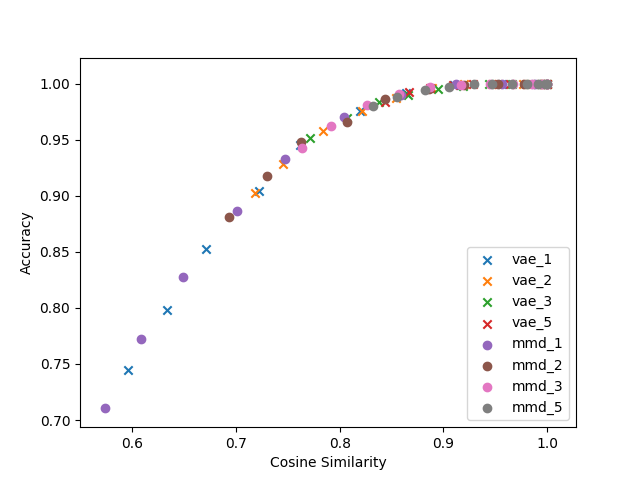
\includegraphics[width=0.7\textwidth]{assets/cos_acc}
    \caption{accuracy vs. cosine similarity for VAE and MMD-VAE based generators at D=20}
\end{figure}

\subsubsection{Objective function score comparison and sample generations}

By progressively allowing for finer tuning of the $\theta$ hyper-parameter, we find that greater sample variance can be achieved whilst maintaining a high ($>99\%$) accuracy. We partially trained our Medium1 and Medium2 generator using latent space dimension 10 and mmd model. Even at 0.01\% completion, we discovered optimizing $\theta$ vector above the Cosine-Accuracy curve presented on Figure 1. Table 4 summarizes our results. \par

\begin{table}[h]
  \caption{$\theta$ and $n$ Parameters (*partial results)}
  \label{theta}
  \centering
  \begin{tabular}{lllll}
    \toprule
    VAE     & Generator     & $\theta$ / n & $cos(x,x')$ & acc \\
    \midrule
    ELBO-20 & Simple  & 0.4 / 2 & 0.9200 & 0.995 \\
    MMD-20 & Simple &  0.6 / 3  & 0.8870 & 0.9968 \\
    MMD-10 & Medium-1 & [0.  0.  0.2 0.2 0.4 0.4 0.4 0.4 0.4 0.8]* & 0.8132 & 0.9980 \\
    MMD-10 & Medium-2 & Not shown & 0.7075 & 0.9999 \\
    \bottomrule
  \end{tabular}
\end{table}

Finally, for each of the 3 optimized configurations, we demonstrate the respective generators' ability to conditionally generate samples on Figures 2-4. In particular, using the Medium-1/2 generators allows us to obtain comparable picture quality even at half the dimension size of the Simple generated samples, and the samples exhibited show greater variety.
\begin{figure}[htb]
\minipage{0.49\textwidth}
  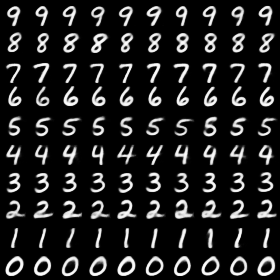
\includegraphics[width=\linewidth]{assets/elbo_20_simple.png}
  \caption{ELBO-VAE / Latent-Dim=20 / Simple Gen}\label{fig:elbo_20_simple}
\endminipage\hfill
\minipage{0.49\textwidth}
   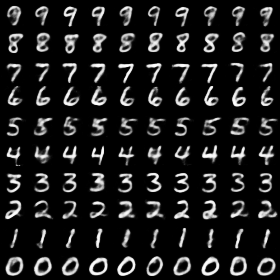
\includegraphics[width=\linewidth]{assets/mmd_20_simple.png}
  \caption{MMD-VAE / Latent-Dim=20 / Simple Gen}\label{fig:mmd_20_simple}
\endminipage\hfill
\minipage{0.49\textwidth}%
   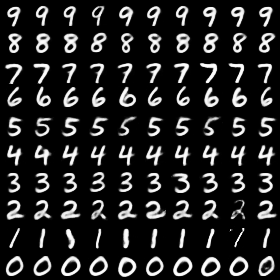
\includegraphics[width=\linewidth]{assets/mmd_10_medium.png}
  \caption{MMD-VAE / Latent-Dim=10 / Medium1 Gen}\label{fig:mmd_10_medium}
\endminipage\hfill
\minipage{0.49\textwidth}
   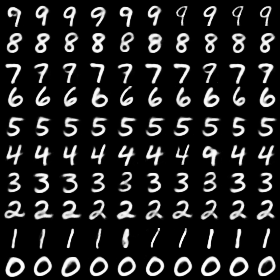
\includegraphics[width=\linewidth]{assets/mmd_10_medium2.png}
  \caption{MMD-VAE / Latent-Dim=10 / Medium2 Gen}\label{fig:mmd_20_simple}
\endminipage
\end{figure}
\section{Related Works}
\label{sec:related}
\subsection{Attribute2Image}

Attribute2Image is a multimodal variational autoencoder \cite{Yan}. It separates the foreground and background into two VAEs for training and merge the image through a gated layer at the end. 
\begin{equation} 
x=x_F + x_B \odot g
\end{equation}
The disentangled latent variables represented by $z=[x_F, x_B]$ can be combined to generated realistic and diverse samples. The highly compressed latent layer for the foreground and background can encode attributes such as lighting, viewpoint and hair color, gender respectively. Our method can augment the robustness of this work by providing a scheme to analyze the distributions of each encoded attribute.

\subsection{MusicVAE}

MusicVAE is a project by Google's Magenta research team to create a variational autoencoder for music \cite{Roberts}. Although VAE models have been shown to be effective models for producing semantically meaningful representations of natural data, especially as it pertains to images, not much work had been done to bring these advances to music effectively. Since music derives its meaning from sequences of long term structures, MusicVAE addresses this issue by using a hierarchical decoder that is based on existing architectures for recurrent VAE models. Additionally, MusicVAE explores the space between different musical sequences using interpolation between latent vectors to generate novel examples that exist in latent space between two example musical pieces given as inputs. Furthermore, MusicVAE explores the identification of 'attribute vectors'. These vectors aim to codify different features inherent in the music analyzed and which allow one to use arithmetic to add or subtract those features, with some success, from a given musical sequence. By analyzing the structure of musical sequences via latent representations, MusicVAE paves way for understanding the distinguishing properties of different genres and themes.

\subsection{Generative Adversarial Networks}

Generative Adversarial Networks (GAN) are a deep neural net architecture comprised of two networks, a discriminator (Dis) and a generator (Gen) set up against each other. Introduced in 2015 \cite{Mirza}, GANs leverage the concept of a 2-player min-max game from Game Theory to set up a network where the Discriminator and Generator are each trying to fool each other. In the process the Generator should learn the underlying distribution of the data space so that it can generate new examples that can fool the discriminator, while the discriminator should learn to discriminate fake examples generated by the Generator from real examples.\par
In this process the GAN aims to maximize/minimize the binary cross entropy of the network:
\begin{equation} 
L_{GAN}=\log(Dis(x))+\log(1-Dis(Gen(z)))
\end{equation}
Where x is a real example from data space and z is a random latent vector fed as input into the Generator. The generator is ultimately trying to learn p(z). The discriminator assigns probability y = Dis(x)  to the event that x is a real training sample and 1 - y to the probability that the input x was generated by Gen. Extensions on existing work on GANs like ConditionalGAN explore ways in which GANs can be trained to conditionally generate examples depending on the desired feature values \cite{Mirza}. Whilst GAN-based conditional generators have advantage over our proposed method in generating a more diverse, high fidelity generations, they also require much heavier computing resources, and in simpler problem settings, we argue that our method is robust enough to fit the needs.

\section{Conclusion}

In this paper we have shown that, by relatively simple analysis of the label-specific distributions in latent space, it is possible to construct a statistical generator capable of generating artificial samples of specific type whilst maintaining variance of the samples generated. Whilst our results are preliminary, our work presents an alternative to generators based on complex neural network models, have added advantage of being consisted of self-contained replaceable components, allowing us to replace each component with state-of-the-art alternatives. In the future, a possible extension would be to improve the generator component using Bayes net to further exploit relationship between distributions of each feature in the latent space, and/or use further heuristics to improve training velocity. 

\medskip

\bibliography{bibl}
\bibliographystyle{plain}
\end{document}
